\chapter{Анализ состояния теоретических исследований и практических разработок современных электроприводов на базе синхронных двигателей с постоянными магнитами } \label{ch:ch1}

\section{Топологии электромобилей} \label{sec:ch1/sec1}

%Мы можем сделать \textbf{жирный текст} и \textit{курсив}.
Электромобили в настоящее время рассматриваются как наиболее перспективный вид транспортного средства. Причиной этому служит ряд его преимуществ: Отсутствие вредных выбросов во время движения, низкий шум, а также высокий крутящий момент на старте. Однако, на данный момент, электромобили сильно уступают транспортным средствам с двигателями внутреннего сгорания (ДВС) по максимальному запасу хода. В условиях ограниченного запаса емкости аккумуляторных батарей (АБ) на борту электромобиля возникает необходимость в разработке наиболее энергоэффективной, легкой и компактной тяговой установки, чтобы увеличить максимальный запас хода электромобиля на одном заряде. 
На данный момент можно выделить два основных способа достичь максимального значения удельной мощности (отношения сумм мощностей тяговых агрегатов к конечному весу автомобиля) и максимальной эффективности трансмиссии электромобиля. Первый способ (рисунок \ref{fig:nomr}) заключается в установке высокоскоростного электромотора (так как их вес и габариты существенно ниже, чем у моторов с более низкой скоростью и эквивалентной мощностью). Однако недостатком такого способа является наличие механических потерь в трансмиссии, что сильно снижает общую эффективность топологии.
Более простым и эффективным способом повышения удельной мощности транспортного средства является использование мотор-колес: высоко-моментных, низкоскоростных моторов, установленных внутри колес автомобиля (рисунок \ref{fig:mr}). Подробно данный тип электромоторов был рассмотрен в \cite{1Luque}[1]. Использование мотор-колес в трансмиссии электротранспорта позволит достичь улучшения динамических характеристик электротранспорта, а также избавиться от таких частей трансмиссии как карданный вал, дифференциал и т.д. Это позволит снизить конечный вес агрегата, а также повысить общий КПД системы \cite{2KingJetTseng,3Lovatt}.
\noindent К основным достоинствам использования мотор-колес можно отнести::
\begin{enumerate}
	\item Независимое управление моментом и скоростью каждого колеса.
	\item Оптимизация места (более компактное расположение).
	%\item Третий пункт.
\end{enumerate}
На данный момент автомобили с мотор-колесами разрабатываются многими производителями \cite{4Jain,5Espanet}, в том числе в условиях бездорожья \cite{6Zhitkova}.
\begin{figure}[ht]
	\centering
	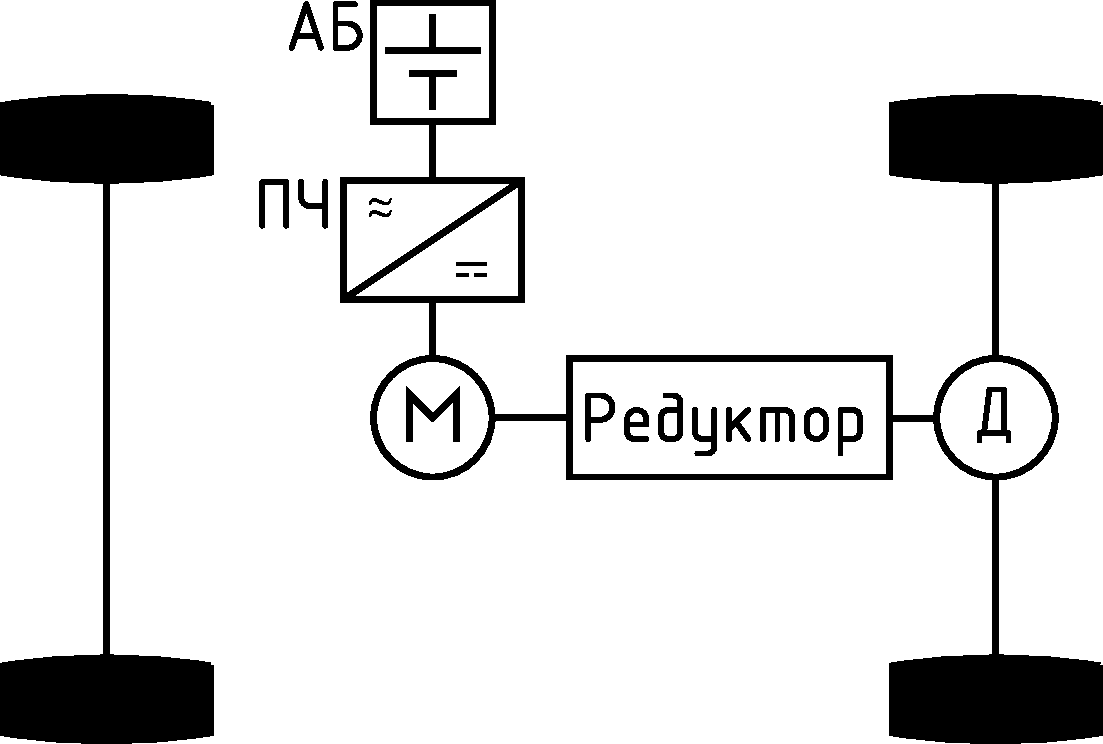
\includegraphics [scale=0.5] {nomr}
	\caption{Стандартная топология электротрансмиссии с одним мотором \cite{4Jain}}
	\label{fig:nomr}
\end{figure}


\begin{figure}[ht]
	\centering
	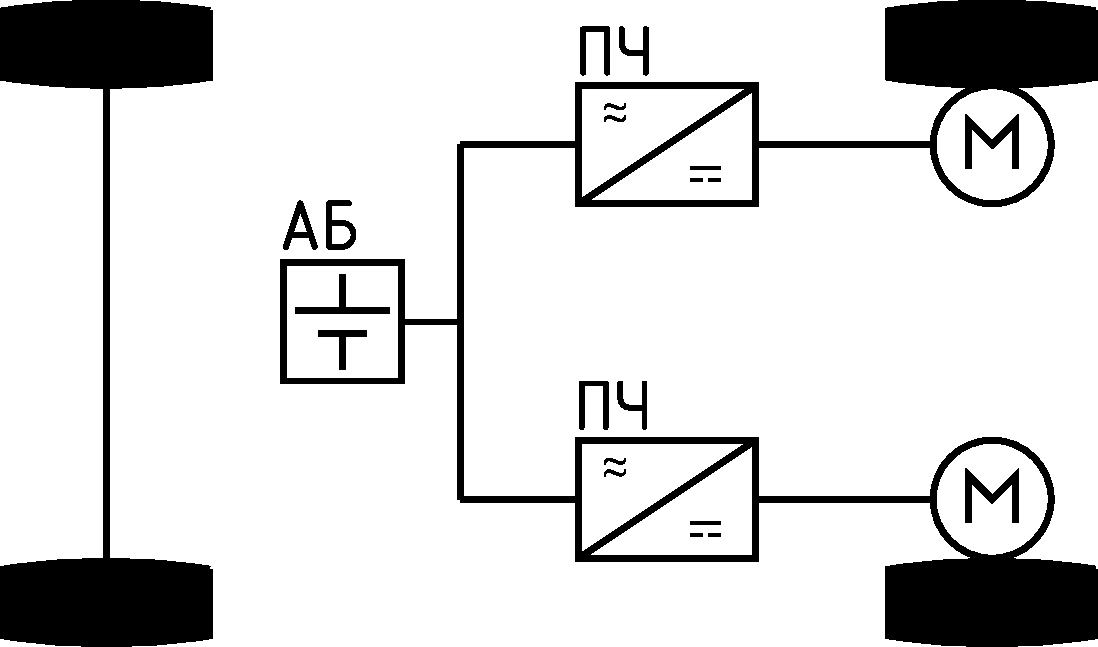
\includegraphics [scale=0.5] {mr}
	\caption{Топология электротрансмиссии с мотор-колесами \cite{4Jain}}
	\label{fig:mr}
\end{figure}

На рисунке \ref{fig:inwheel} изображено мотор-колесо, разработанное компанией Protean, а также его составные части. 
Однако, несмотря на вышеперечисленные достоинства, данный тип моторов имеет один недостаток – большая неподрессоренная масса, которая снижает комфорт от езды, а также уменьшает способность автомобиля удерживать заданное направление движения. Существуют различные способы решения данной проблемы \cite{7Tang}, однако их решение выходит за рамки поставленных в исследовании целей и задач.

\begin{figure}[ht]
	\centering
	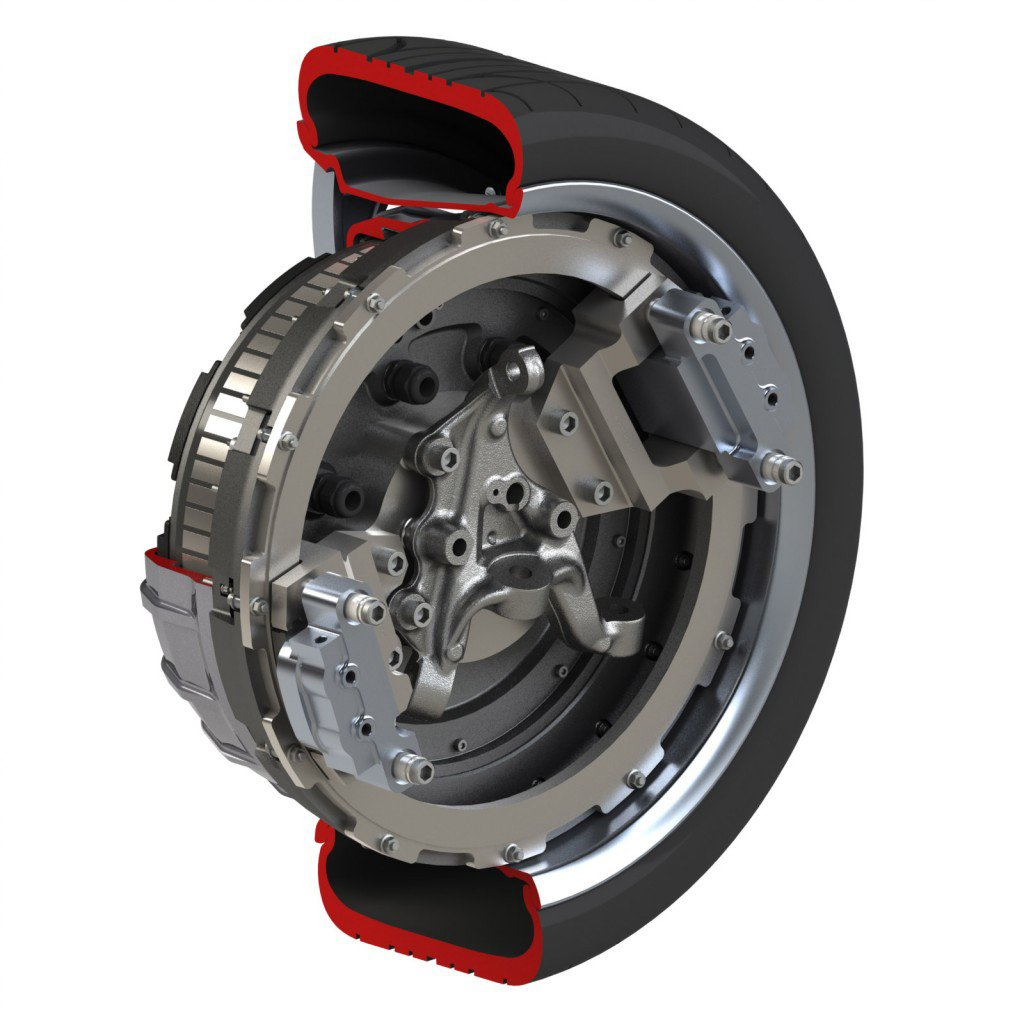
\includegraphics [scale=0.25] {inwheel}
	\caption{Мотор-колесо}
	\label{fig:inwheel}
\end{figure}

В составе мотор-колеса могут быть использованы различные типы электродвигателей. Данное исследование ориентировано на рассмотрение мотор-колес с синхронным электродвигателем с постоянными магнитами (СДПМ). Ниже будут рассмотрены основные достоинства и недостатки СПДМ в составе мотор-колес. 

\section{Мотор-колеса в составе автомобиля} \label{sec:ch1/sec2}
\noindent Основными требованиями для электромоторов в составе мотор-колес являются:
\begin{enumerate}
	\item Высокий крутящий момент на низких скоростях
	\item Широкий диапазон регулирования скорости
	\item Высокий коэффициент удельной мощности
\end{enumerate}

Низкий вес мотора – наиболее важный параметр, необходимый для достижения высоких динамических характеристик мотора вследствие уменьшения общей неподрессоренной массы электромобиля. Таким образом отношение КПД мотора к его весу – основной критерий выбора электромотора. \noindent Электродвигатели, соответствующие вышеобозначенным критериям, представлены следующими типами:
\begin{enumerate}
\item Асинхронный электродвигатель \cite{8Benoudjit,9FeiXu}
\item Синхронный двигатель с постоянными магнитами \cite{10Fan}
\item Бесщеточный двигатель постоянного тока (вентильный электродвигатель) \cite{11YeePienYang,12Miyamasu}
\item Вентильный реактивный электродвигатель \cite{13Luk}
\end{enumerate}
Подробный анализ и сравнение различных типов электромоторов выходит за рамки поставленных в исследовании целей и задач. Работы, в которых проводится обозначенное исследование представлены в \cite{15Nanda}. Как было обозначено ранее, представленное исследование рассматривает СДПМ в качестве тягового электромотора в составе мотор-колес, так как данный тип электродвигателей имеет высокий коэффициент удельной мощности, низкую инерционность ротора, высокий крутящий момент на низких скоростях, Высокий КПД (благодаря отсутствию обмоток в роторе)
\section{Типы синхронных двигателей с постоянными магнитами} \label{sec:ch1/sec3}

Синхронный электродвигатель с постоянными магнитами, как и любой вращающийся электродвигатель, состоит из ротора и статора. Статор - неподвижная часть, ротор - вращающаяся часть. Обычно ротор располагается внутри статора электродвигателя, также существуют конструкции с внешним ротором - электродвигатели обращенного типа (рисунок \ref{fig:mr}).

\begin{figure}[ht]
	\centering
	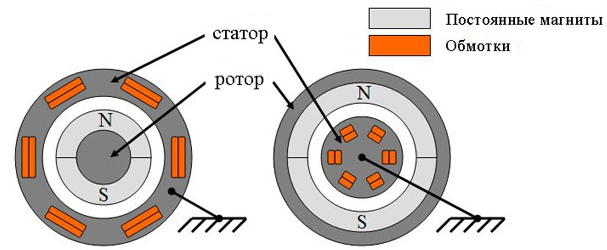
\includegraphics [scale=1] {intoutrot}
	\caption{Конструкции синхронного двигателя с постоянными магнитами: слева - стандартная, справа обращенная.}
	\label{fig:intoutrot}
\end{figure}

Ротор состоит из постоянных магнитов. В качестве постоянных магнитов используются материалы с высокой коэрцитивной силой.

\noindent По конструкции ротора синхронные двигатели делятся на:
\begin{enumerate}
\item электродвигатели с явно выраженными полюсами;
\item электродвигатели с неявно выраженными полюсами.
\end{enumerate}

Электродвигатель с неявно выраженными полюсами имеет равную индуктивность по продольной и поперечной осям $L_{d} = L_{q}$, тогда как у электродвигателя с явно выраженными полюсами поперечная индуктивность не равна продольной $L_{d} \neq L_{q}$.

\begin{figure}[ht]
	\centering
	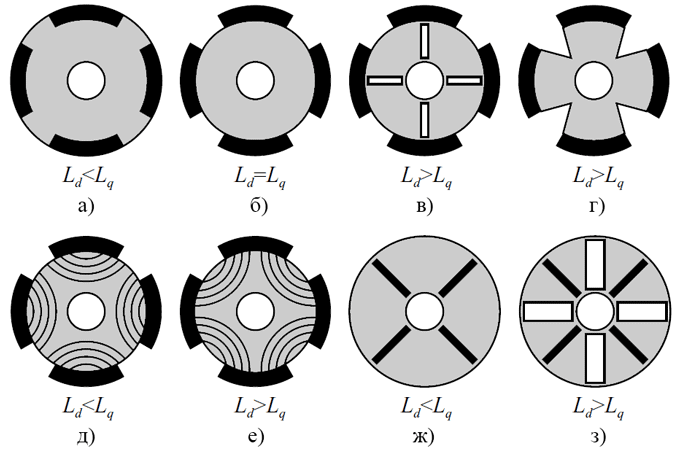
\includegraphics [scale=0.7] {rotor_saliency}
	\caption{Сечение роторов с разным отношением Ld/Lq. Черным обозначены магниты. На рисунке д, е представлены аксиально-расслоенные роторы, на рисунке в и з изображены роторы с барьерами.}
	\label{fig:rotor_saliency}
\end{figure}

Также по конструкции ротора СДПМ делятся на:
синхронный двигатель c поверхностной установкой постоянных магнитов
(англ. SPMSM - surface permanent magnet synchronous motor);
синхронный двигатель со встроенными (инкорпорированными) магнитами
(англ. IPMSM - interior permanent magnet synchronous motor).


\begin{figure}[ht]
	{\centering
		\hfill
		\subbottom[List-of-Figures entry][\label{fig:rotor_spmsm}]{%
			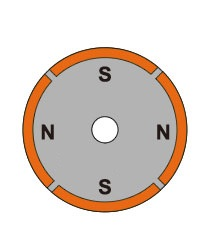
\includegraphics[width=0.35\linewidth]{rotor_spmsm}}
		\hfill
		\subbottom[\label{fig:rotor_ipmsm}]{%
			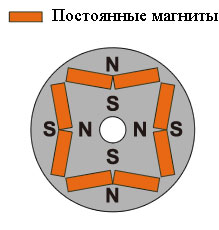
\includegraphics[width=0.35\linewidth]{rotor_ipmsm}}
		\hfill
	}
	\legend{а) Ротор синхронного двигателя c поверхностной установкой постоянных магнитов; б) Ротор синхронного двигателя со встроенными магнитами.}
	\caption{Конструкции ротора СДПМ}
	\label{fig:rotor_pmsm}
\end{figure}

Статор состоит из корпуса и сердечника с обмоткой. Наиболее распространены конструкции с двух- и трехфазной обмоткой.

\noindent В зависимости от конструкции статора синхронный двигатель с постоянными магнитами бывает:
\begin{itemize}
\item с распределенной обмоткой;
\item с сосредоточенной обмоткой.
\end{itemize}

Распределенной называют такую обмотку, у которой число пазов на полюс и фазу $Q = 2, 3,...., k$.
Сосредоточенной называют такую обмотку, у которой число пазов на полюс и фазу $Q = 1$. При этом пазы расположены равномерно по окружности статора. Две катушки, образующие обмотку, можно соединить как последовательно, так и параллельно. Основной недостаток таких обмоток - невозможность влияния на форму кривой ЭДС.
Представленное исследование рассматривает в качестве объекта синхронные двигатели с постоянными магнитами с поверхностной установкой постоянных магнитов (англ. SPMSM) и концентрированной обмоткой, так как данный тип моторов является наиболее подходящим для электротранспорта по следующим критериям: 

\begin{itemize}
\item Высокие энергетические показатели (КПД более $90\%$)
\item Меньшие масса и габариты в сравнении с остальными типами электромоторов при одинаковой мощности
\item Широкий диапазон изменения частоты вращения
\item Высокая перегрузочная способность по моменту
\item Большой срок службы и высокая надежность
\end{itemize}

В отличии от СДПМ с распределенной обмоткой, электромотор с концентрированной имеет более низкий вес (так как распределенная обмотка укладывается "в нахлест"), что особенно важно, так как конечный вес электромобиля напрямую влияет на запас хода на одном заряде и, как следствие, на эффективность работы всей системы в целом

\section{Методы управления синхронными двигателями с постоянными магнитами} \label{sec:ch1/sec4}

Интерес к вопросу регулирования координат синхронного двигателя прослеживается в течение последних десятков лет. Многие авторы проводили разработку и исследование различных типов синхронных двигателей с постоянными магнитами.

В 1986 г. Джахнс T.M., Климан Г.Б. и Нейманн T.В. [62] показали, что использование постоянных магнитов в синхронных двигателях с явновыраженными полюсами для регулируемых электроприводов улучшают их характеристики по отношению к другим классам машин переменного тока. Они надёжнее, способны обеспечить большую мощность при относительно малых габаритах, могут работать на высоких скоростях в двигательном и генераторном режимах, энергетически эффективны в широком диапазоне скоростей.
В 1986 году Себастьяном T., Слемоном Г. и Рахманом M.[109] были рассмотрены перспективы развития электроприводов на базе СДПМ и представлены эквивалентные модели электрических схем для таких двигателей, а также методы определения их параметров. Сравнение результатов моделирования с проведенными экспериментами подтвердило адекватность их модели. 

Пиллэй П. и Кришнан Р. [96 - 98] классифицировали синхронные двигатели на два типа: синхронные двигатели с 19 постоянными магнитами (СДПМ) и бесщеточные двигатели постоянного тока (БДПТ). СДПМ имеет синусоидальную противоЭДС и для него нужно формировать синусоидальный ток статора для получения постоянного крутящего момента, а БДПТ имеет трапецеидальную противо-ЭДС и работает с прямоугольными токами статора для получения постоянного крутящего момента. СДПМ очень похож на синхронный двигатель с неявновыраженными полюсами, у которого вместо обмотки возбуждения используется постоянный магнит.

Модель СДПМ может быть получена из хорошо известной модели синхронной машины. Уравнения СДПМ выводятся в $d-q$ системе координат, жёстко связанной с ротором. Обмотка возбуждения из модели исключается в силу ее отсутствия, а поток ротора считается постоянным, в силу особенности расположения системы координат. 
Представление уравнений СДПМ в системе координат $d-q$ является основным способом описания его работы. Такое описание обеспечивает наглядность протекающих в обмотках статора процессах. Действительные токи и напряжения статора в приведенной двухфазной неподвижной системе координат связаны с роторными величинами однозначным преобразованием. Эти преобразования основаны на предположении о симметричности электрических и магнитных цепей всех обмоток. Кроме системы координат $d-q$ иногда применяется система координат $\alpha-\beta$, при этом значение индуктивности обмоток статора связано тригонометрическими зависимостями с угловым положением ротора. 
Существует также пространственная модель СДПМ учитывающая потери энергии [54, 75, 83, 85, 120]. На базе этой 20 модели были предложены методы оценки изменяющихся параметров двигателя в процессе работы. 

Модели различных типов синхронных двигателей в сравнении с асинхронными двигателями приведены в [99, 109, 117], где получена модель основных полюсов синхронного двигателя, а все уравнения выведены в системе координат $d-q$ и представлены в виде матрицы. Эквивалентная схема двигателя при этом включала демпфирующую обмотку и была представлена как источник постоянного тока. 

Разработанные в 80-х годах прошлого века математические модели СДПМ впоследствии были реализованы в виде компьютерных программ, в том числе и в виде блоков среды Matlab Simulink, эффективность и адекватность которых отмечается во многих работах [55, 74, 91, 92, 106]. 
Электропривод на базе СДПМ, как объект управления, не имеет существенных отличий от электропривода на базе синхронного двигателя с обмоткой возбуждения расположенной на индукторе, поэтому и методы управления синхронным двигателем приемлемы и для СДПМ.
 
Развитие принципов управления электропривода с СДПМ обуславливается развитием теории и методов управления, а также совершенствованием аппаратной базы электропривода. Реализация управления СДПМ с учетом параметров самого двигателя, наличием датчиков углового положения ротора, типом преобразователя и вычислительной мощностью контроллера позволяет судить об эффективности используемых алгоритмов [22]. 

Один из первых способов управления синхронными двигателями на базе полупроводникового преобразователя получил название вентильного двигателя [6, 33, 57, 58, 67, 87, 111, 21 114, 115], который также называют бесколлекторным двигателем постоянного тока с возбуждением от постоянных магнитов. Учитывая, что коммутация ключей вентильного двигателя жестко связана с положением ротора, напряжение, прикладываемое к фазам двигателя при его работе, имеет трапецеидальную форму. Данный способ управления достаточно прост в реализации и имеет хорошее быстродействие, но ему присущи большие пульсации момента. 
Для повышения качества управления современные СДПМ, как правило, питаются от автономного инвертора напряжения, формирующего в соответствии с текущим состоянием двигателя вектор напряжения, необходимый для достижения цели управления. 

При формировании вектора напряжения можно добиться распределения потока статора близкого к синусоидальной форме, поэтому для СДПМ нашли применение те же методы управления, которые используются для асинхронных двигателей [7, 10, 18, 21]. К таким методам в первую очередь относятся полеориентированное управление и прямое управление моментом. 
Полеориентированное управление СДПМ рассматривается в работах многих авторов, например [8, 10, 11, 25, 35, 45, 59, 82, 117]. Так, Пиллэй П. и Кришнана Р. в 1989 году [97, 98] показали возможность использования полеориентированного управления применительно к СДПМ. В результате проведенных исследований они показали, что уровень пульсаций электромагнитного момента при полеориентированном управлении существенно меньше, чем при использовании алгоритмов управления вентильным двигателям с датчиками Холла. 
Моримото С., Тонг И., Такеда И. и Хираса Т. в 1994 г. [85] и Мадемлис C., Маргарис Н. в 2002 г. [75] представили работы по 22 созданию алгоритмов управления СДПМ, направленных на улучшение энергетической эффективности путем оптимизации потерь в меди и стали статора, на базе системы полеориентированного управления. 
Общим недостатком всех рассматриваемых систем полеориентированного управления СДПМ является невысокое быстродействие регулирования момента по сравнению с прямым управлением моментом (ПУМ), что сужает область их применения в высокоточных динамичных электроприводах. 

В электроприводах, требующих высокого быстродействия регулирования, получили распространение СДПМ с прямым управлением моментом. Основным принципом прямого управления моментом является выбор соответствующего вектора напряжения в зависимости от положения вектора магнитного потока ротора, разницы между заданным и реальным крутящим моментом [30, 39, 48, 49, 56, 59, 60, 61, 64, 78, 79, 80, 90, 93, 99, 102, 103, 104, 117, 122, 127, 128].

ПУМ может быть реализовано без датчиков [42, 84, 94, 100, 105, 113, 117], если известно первоначальное положение ротора. Так, Юоон-Хо Ким, Юоон-Санг Коок в 1999 году [125], предложили эффективные методы определения положения ротора, информация о котором необходима для пуска двигателя.

Прямое управление моментом имеет такие преимущества, как хорошее быстродействие по моменту, высокий электромагнитный момент при низких скоростях. Однако работа электропривода с ПУМ сопровождается высокими пульсациями электромагнитного момента, особенно на низких скоростях. По этой причине работы многих авторов направлены на снижение уровня таких пульсаций [41, 67, 71, 77, 81, 95, 115, 118, 119, 121, 123, 124, 125]. Например, в работе [67] представлены таблицы переключений для прямого управления моментом, использование которых способствует снижению уровня пульсаций. Там же рассмотрена конструкция наблюдателя, позволяющая при прямом управлении моментом проводить оценку положения ротора и момента сопротивления на валу двигателя. 

Помимо полеориентированного и прямого управления моментом, для систем управления электроприводов с СДПМ могут использоваться и другие способы, основанные на применении теории автоматического управления. Например, в работе [13] рассматривается применение метода скоростного градиента, а в [32, 34] теории синергетического управления. Данные работы имеют в качестве недостатка невысокое быстродействие. В [43, 50, 53, 57, 66, 68, 73, 122] рассматривается применение скользящих режимов для управления СДПМ, отличительной особенностью которых является возможность потери устойчивости работы, а также высокие пульсации электромагнитного момента. 
С целью обеспечения повышенных скоростей при работе с малыми нагрузками в [63, 65, 76, 86, 116] предложены алгоритмы управления позволяющие ослаблять главный магнитный поток. Исследования, проведенные авторами показали робастность системы управления по отношению к параметрам двигателя и устойчивую работу при переходах от номинального потока к ослабленному и обратно, с высоким быстродействием. 

Широкое распространение получило применение интеллектуальных методов управления, таких как нейронные сети [51, 52, 70, 101], нечеткая логика [40, 46, 48, 56, 60, 67, 79, 89, 108], генетические алгоритмы и т.п., как самостоятельные способы управления, так и в сочетании с полеориентированным или прямым управлением моментом.
Так, на основе генетических алгоритмов в [126] предложен подход к управлению СДПМ, который предусматривает определение параметров ПИД-регулятора, гарантирующих надежную устойчивость замкнутой системе. 

В [84] на базе систем управления с переменной структурой с использованием повторяющегося обучения рассмотрен подход к минимизации периодических пульсаций скорости СДПМ. Эти пульсации скорости вызваны пульсациями электромагнитного момента, которые изменяются периодически в зависимости от положения ротора. Обычный П-регулятор скорости имеет возможность уменьшить рассмотренные пульсации скорости до определённого уровня, но недостаточного для многих высокопроизводительных приложений. В установившемся состоянии система управления с переменной структурой с использованием повторяющегося обучения вырабатывает задание для компенсации текущих пульсаций, что вместе с внешним контуром регулирования скорости используется для уменьшения пульсаций скорости. Предлагаемый способ управления может быть легко интегрирован в любую из существующих систем электропривода с СДПМ. 

Еще одной работой, предлагающей нестандартный регулятор скорости, является [110], где применяется модульный подход к управлению скоростью СДПМ. На основе функционирования отдельных регуляторов, модульный подход позволил реализовать интеллектуальный и надежный регулятор, который позволяет легко заменить любой существующий регулятор, работающий недостаточно качественно, сохранив другие регуляторы, которые эффективны. Впервые был проведен анализ устойчивости пропорционально-интегрального (ПИ) регулятора скорости в обычной системе управления СДПМ. Затем было показано, что обычные регуляторы СДПМ не могут исключить пульсации электромагнитного момента, которые были основным препятствием использования СДПМ в качестве высокопроизводительного сервопривода. В предложенных регуляторах это было достигнуто путем введения модуля с итерационным обучением. Этот модуль осуществляет циклическую запись момента и текущих сигналов управления за один полный цикл, а затем использует эти сигналы для обновления текущего задания на следующий цикл. Как следствие, пульсации крутящего момента могут быть значительно снижены. Для того чтобы оценить пульсации момента, также был предложен модуль оценки, использующий скользящие режимы. Наблюдатель получил дальнейшее развитие в целях содействия осуществлению регулирования момента. Предлагаемая система управления была оценена моделированием в режиме реального времени и экспериментальными результатами, которые подтвердили ее эффективность.
Достаточно мощным направлением в развитии электроприводов на базе СДПМ является построение бездатчиковых систем, позволяющих отказаться от применения дополнительных механических устройств, устанавливаемых на валу двигателя. Основными оцениваемыми координатами в таких электроприводах являются скорость и угловое положение ротора. Для построения наблюдателей используется большое многообразие различных подходов. 

Одним из таких подходов является применение расширенного фильтра Калмана [44, 125], который позволяет производить оценку параметров и переменных величин двигателя в условиях случайного характера внешних воздействий. Так, в [72, 88] приведена оценка скорости, положения ротора и момента 26 нагрузки при прямом управлении моментом СДПМ на основе расширенного фильтра Калмана. Разработана модель СДПМ и фильтра Калмана в Matlab Simulink. Предлагаемые наблюдатели скорости оказались нечувствительными к изменениям параметров двигателя. Результаты моделирования продемонстрировали хорошую производительность и надежность. Недостатком таких систем является необходимость в использовании существенных вычислительных ресурсов контроллера. 

Еще одним вариантом построения бездатчиковых электроприводов на базе СДПМ являются адаптивные системы [47, 66, 107]. Например, широко распространено применение адаптивной системы с настраиваемой моделью, однако для этих систем так же существенным недостатком является большая вычислительная нагрузка на контроллер. 
Распространенным является применение наблюдателей состояния [72, 88, 112]


\section{Выводы по главе} \label{sec:ch1/sec5}

 Результаты проведённого анализа состояния теоретических исследований и практических работ показали, что:
\begin{enumerate}
\item Трансмиссия электротранспорта с использованием мотор-колес является наиболее перспективным решением, так как её использование позволяет снизить конечный вес электромобиля, а также повысить общий КПД системы. 
\item Благодаря весьма благоприятным свойствам по виду механических и регулировочных характеристик, отсутствию скользящих электрических контактов, отсутствию потерь на возбуждение и возможностям эффективного охлаждения, СДПМ является наиболее перспективным электродвигателем для использования в составе мотор-колес.
\item Применение современных магнитотвердых материалов позволило создавать СДПМ, способные конкурировать по массогабаритным и энергетическим показателям с машинами с электромагнитным возбуждением в широком диапазоне мощностей и частот вращения, а по удельному показателю как величина электромагнитного момента на единицу массы СДПМ практически нет равных среди разнообразных типов электрических двигателей.
\item Наиболее распространёнными для построения систем управления электроприводов на базе СДПМ являются полеориентированное управление и прямое управление моментом.
\item Наибольшим быстродействием из этих двух способов обладает прямое управление моментом, что позволяет использовать его в высокоточных и динамичных электроприводах, в которых требуется высокое быстродействие.
\item Для работы системы электропривода с СДПМ в составе мотор-колеса необходимо достижение широкого диапазона скоростей, поэтому необходимо адаптировать алгоритм СДПМ для работы в режиме ослабленного поля.
\end{enumerate}
\noindent Исходя из этого, можно сформулировать следующие основные задачи, решаемые в работе:
\begin{enumerate}
\item На базе разработанной имитационной модели электропривода с СДПМ проанализировать возможность увеличения диапазона рабочих скоростей за счет работы СДПМ в режиме ослабленного поля.
\item Проанализировать влияние времени дискретизации системы управления электроприводом и параметров СДПМ на величину пульсаций электромагнитного момента.
\item Разработать алгоритмы управления электроприводом с СДПМ, обеспечивающие быстродействие соизмеримое с системами прямого управления моментом при уровне пульсаций, характерном полеориентированному управлению.
\item Оценить адекватность математической модели, используемой при синтезе и анализе системы управления, путем экспериментальных исследований с учётом особенностей технической реализации системы управления электроприводом с СДПМ.
\end{enumerate}